\hypertarget{aaron-r-miller}{%
\section{Aaron R Miller}\label{aaron-r-miller}}

A highly professional software developer with over 12 years of
experience

\begin{figure}
\centering
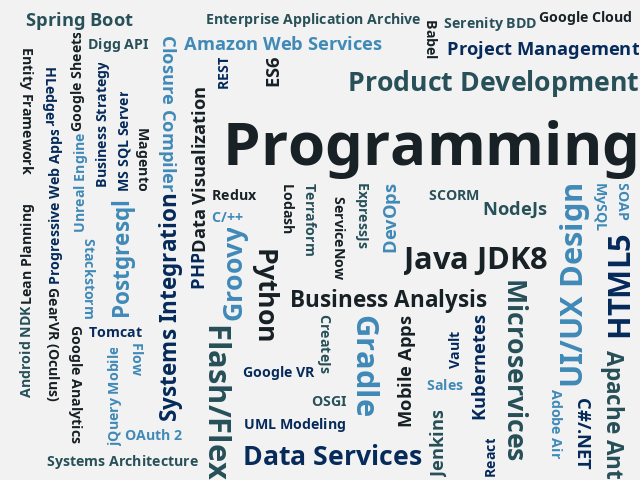
\includegraphics{img/skillcoud-1.0.0.png}
\caption{Skill Cloud Diagram}
\end{figure}

\textbf{Objective}

Seeking new opportunities to develop software remotely as a 1099, C2C,
or W2 contractor

\hypertarget{work-experience}{%
\subsection{Work Experience}\label{work-experience}}

\hypertarget{cartoonifyit-open-source-feb-2020---current}{%
\subsubsection{CartoonifyIt @ Open Source (Feb 2020 -
CURRENT)}\label{cartoonifyit-open-source-feb-2020---current}}

Developed Augmented Reality (AR) demo with Rust and Android NDK (in
progress) https://github.com/drkstr101/CartoonifyIt

\begin{itemize}
\tightlist
\item
  Ported the C++ Android NDKCamera sample app to Rust
\item
  Created standalone crate to extend android-ndk with added support for
  NDKCamera FFI bindings
\end{itemize}

\emph{Programming, Mobile Apps, C/++, Rust, FFI, Android NDK}

\hypertarget{earthnew.media-open-source-feb-2020---current}{%
\subsubsection{earthnew.media @ Open Source (Feb 2020 -
CURRENT)}\label{earthnew.media-open-source-feb-2020---current}}

Developing federated social media app from scratch as a teaching tool to
help a friend learn to program (in progress)
https://gitlab.com/earthnewmedia

\begin{itemize}
\tightlist
\item
  Produced project inception document with business case and specs for a
  1.0 MVP release
\item
  Implemented BDD style test suite for integration testing between
  decoupled web projects
\item
  Created RESTful API with JWT client security for backend CRUD services
  and SPA for prototype UX
\end{itemize}

\emph{Programming, UI/UX Design, Domain Modeling, Product Development,
Business Analysis, Mentor, NodeJs, React, Redux, SagasJs, Bootstrap,
HTML5, REST, Serenity BDD, Typescript, Loopback 4}

\hypertarget{waweb-site-plugin-open-source-nov-2019---current}{%
\subsubsection{WaWeb Site Plugin @ Open Source (Nov 2019 -
CURRENT)}\label{waweb-site-plugin-open-source-nov-2019---current}}

Developed a collection of integrated Gradle plugins for static website
development and publication https://gitlab.com/waweb/waweb-site-plugin
(ref 200-beta)

\begin{itemize}
\tightlist
\item
  Created suite of Gradle plugins, including support for JavaScript
  compilation, SASS, and extended Groovy Template Engine, with added
  support for markdown to HTML conversion in template definitions
\item
  Developed reusable ``Steps'' library for Serenity BDD to easily test
  multiple Gradle plugins which may interact with each other in a test
  fixture
\end{itemize}

\emph{Programming, JDK, Gradle, Groovy, HTML5, Serenity BDD, Closure
Compiler}

\hypertarget{resume-publisher-open-source-nov-2019---current}{%
\subsubsection{Resume Publisher @ Open Source (Nov 2019 -
CURRENT)}\label{resume-publisher-open-source-nov-2019---current}}

Developed Gradle plugin which publishes an html and docx format of my
resume https://gitlab.com/aaron.miller/resume/

\begin{itemize}
\tightlist
\item
  Created Resume domain model and GUI editor using the Eclipse ECore
  modeling tools
\item
  Created Gradle plugin which adds builder support and publishing
  capabilities for the Resume model, with outputs including an XMI data
  exchange format, static html site stylized docx,and ``Word Cloud''
  image generation from skills listed in the model.
\end{itemize}

\emph{Programming, UI/UX Design, Domain Modeling, EMF/ECore, jQuery
Mobile, Gradle, Groovy, JDK, HTML5, OOXML}

\hypertarget{ctoco-owner-washington-web-apps-aug-2019---current}{%
\subsubsection{CTO/Co-Owner @ Washington Web Apps (Aug 2019 -
CURRENT)}\label{ctoco-owner-washington-web-apps-aug-2019---current}}

Co-founder and chief technical lead at a software development
consultancy

\hypertarget{business-development}{%
\paragraph{Business Development}\label{business-development}}

\begin{itemize}
\tightlist
\item
  Developed and produced a majority of the Lean Business Plan document,
  including an initial target market, product, sales/marketing, and
  pricing strategies
\item
  Identified talents and negotiated partnerships to fill the roles of
  CFO and COO, to delegate responsibilities for legal, accounting,
  business development and growth
\item
  Developed a basic reproducible sales process as a starting point used
  to train and onboard the COO, aiding them in the pursuit of sales
  growth
\end{itemize}

\emph{Product Development, Business Analysis, Project Management,
Business Strategy, Lean Planning, Sales}

\hypertarget{systems-engineering}{%
\paragraph{Systems Engineering}\label{systems-engineering}}

\begin{itemize}
\tightlist
\item
  Created an append-only accounting system and tooling using a
  combination of plain text files, HLedger, and Git
\item
  Developed proprietary project estimation and pricing tools using the
  Eclipse Modeling Framework (EMF), accounted for as IP Assets in the
  main ledger and providing the primary competitive advantage for the
  company
\end{itemize}

\emph{Programming, Domain Modeling, Terraform, HLedger, Kubernetes, AWS,
Google Cloud, Gradle, Groovy, Spring Boot, JDK, EMF/ECore, HTML5, ES6,
Closure Compiler, Bootstrap}

\hypertarget{systems-engineer-wavsys-jan-2019---aug-2019}{%
\subsubsection{Systems Engineer @ WAVSYS (Jan 2019 - Aug
2019)}\label{systems-engineer-wavsys-jan-2019---aug-2019}}

Staff augmented Systems Engineer at Expedia Group

\begin{itemize}
\tightlist
\item
  Reduced maintenance cost by aiding in the transition of a legacy
  monolith project to a more modern automation framework
\item
  Improved the efficiency of Stackstorm pack development by building and
  maintaining an automated acceptance testing and specification
  framework
\end{itemize}

\emph{Programming, Vault, ServiceNow, Microservices, Kubernetes,
C\#/.NET, Python, Gradle, Stackstorm, Serenity BDD, JDK, Groovy}

\hypertarget{software-developer-catalyte-surge-it-services-aug-2017---aug-2018}{%
\subsubsection{Software Developer @ Catalyte-Surge IT Services (Aug 2017
- Aug
2018)}\label{software-developer-catalyte-surge-it-services-aug-2017---aug-2018}}

Software Engineer at an outsourcing and staff augmentation consultancy
Kadlec Medical Group

\begin{itemize}
\tightlist
\item
  Removed primary blockers and reduced runtime memory footprint by an
  order of magnitude in an Electronic Medical Record (EMR) web
  application Programming, Microservices, REST, NodeJs, HTML5, ES6,
  Babel, Flow, ExpressJs, React, Redux, SagasJs, Domain Modeling Emory
  University
\item
  Developed client-side module and built a release system for custom 2FA
  authentication, when using the AWS Command Line Interface within Emory
  University's internal network
\end{itemize}

\emph{Programming, AWS, Microservices, SOAP, Gradle, Spring Boot, JDK,
Groovy, EAR}

\hypertarget{software-developer-vivid-learning-systems-oct-2010---apr-2017}{%
\subsubsection{Software Developer @ Vivid Learning Systems (Oct 2010 -
Apr
2017)}\label{software-developer-vivid-learning-systems-oct-2010---apr-2017}}

Sr.~Software Engineer for eLearning based products and services company

\hypertarget{sr.-programmer}{%
\paragraph{Sr.~Programmer}\label{sr.-programmer}}

\begin{itemize}
\tightlist
\item
  Developed prototype mobile VR app used by the sales team to entice
  potential customers at trade shows
\item
  Automated workflow for production department and drove the adoption of
  Continuous Integration into the development process
\item
  Designed and developed front end framework to enable the production of
  Computer Aided Learning content as a fully Progressive Web App,
  eliminating the reliance on Flash/Air runtimes in flagship product
\item
  Created prototype data service-oriented back-end architecture that
  supports user authentication and tracking for deployment scenarios
  outside a traditional LMS web portal, later adopted by another team as
  the basis for a rewrite to the backend LMS product
\end{itemize}

\emph{Programming, Mobile Apps, C/++, JDK, Android NDK, Google VR,
GearVR (Oculus), Unreal Engine, Apache Ant, DevOps, Systems Integration,
Groovy, Gradle, Python, Jenkins, OSGI, Microservices, Progressive Web
Apps, HTML5, Closure Compiler, Lodash, jQuery Mobile, CreateJs, NodeJs,
C\#/.NET, MS SQL Server, Entity Framework, Mentor}

\hypertarget{programmer-ii}{%
\paragraph{Programmer II}\label{programmer-ii}}

\begin{itemize}
\tightlist
\item
  Implemented mobile compatible front-end architecture to bring a
  flagship product to the App/Play Store
\item
  Maintained existing flagship product that delivers and tracks the
  usage of rich media content for Computer-Aided Learning
  (``eLearning'')
\end{itemize}

\emph{Programming, Mobile Apps, UI/UX Design, Flash/Flex, Adobe Air,
Python, Apache Ant, SCORM}

\hypertarget{ctoco-owner-open-base-interactive-oct-2008---sep-2010}{%
\subsubsection{CTO/Co-Owner @ Open Base Interactive (Oct 2008 - Sep
2010)}\label{ctoco-owner-open-base-interactive-oct-2008---sep-2010}}

Co-founder and chief technical lead at a software development
consultancy

\hypertarget{nulabel-technologies}{%
\paragraph{NuLabel Technologies}\label{nulabel-technologies}}

\begin{itemize}
\tightlist
\item
  Worked with Director of Science to develop database-driven software
  systems that replaced existing spreadsheet-based workflow in use by
  the lab techs
\end{itemize}

\emph{Product Development, Business Analysis, DevOps, Microservices,
Programming, Mentor, UI/UX Design, JDK, Tomcat, Google Sheets, OAuth 2,
Flash/Flex, Postgresql, Python, Jenkins, Data Visualization, Apache Ant,
Domain Modeling}

\hypertarget{demand-lending}{%
\paragraph{Demand Lending}\label{demand-lending}}

\begin{itemize}
\tightlist
\item
  Designed and developed the software systems for the flagship product
  of a Direct Lending startup
\item
  Managed a team of developers to bring flagship product to market
\end{itemize}

\emph{Product Development, Business Analysis, Project Management,
Systems Architecture, Postgresql, Domain Modeling}

\hypertarget{all-student-rentals}{%
\paragraph{All Student Rentals}\label{all-student-rentals}}

\begin{itemize}
\tightlist
\item
  Created client-server marketplace of rental properties for the winner
  of the ``Best Business Idea'' contest at California State University
\item
  Integrated phone service with back-end systems to automatically detect
  billable leads, through the use of auto-generated extension numbers
  shown in the front-end app, keyed by listing and vendor ID
\end{itemize}

\emph{Product Development, Programming, UI/UX Design, Flash/Flex,
Microservices, Google Analytics, HTML5, Systems Integration, Postgresql}

\hypertarget{ctoco-owner-splash-labs-aug-2007---oct-2008}{%
\subsubsection{CTO/Co-Owner @ Splash Labs (Aug 2007 - Oct
2008)}\label{ctoco-owner-splash-labs-aug-2007---oct-2008}}

Co-founder and chief technical lead at a software development
consultancy

\hypertarget{team08-snowboards}{%
\paragraph{Team08 Snowboards}\label{team08-snowboards}}

\begin{itemize}
\tightlist
\item
  Developed a Fullstack system to enable custom snowboard designs to be
  created and purchased online
\item
  Integrated back-end database systems with CAD manufacturing systems to
  automatically produce working specs from the web-based designer
  utility in the store front-end
\end{itemize}

\emph{Programming, UI/UX Design, Flash/Flex, PHP, Magento, MySQL,
Systems Integration}

\hypertarget{developers-research}{%
\paragraph{Developers Research}\label{developers-research}}

\begin{itemize}
\tightlist
\item
  Created the main company website and simple CMS system for adding or
  removing content Programming, HTML5, PHP Digg Charts
\item
  Created the DiggCharts app which won second place in the Digg.com API
  data visualizations contest
\end{itemize}

\emph{Programming, Flash/Flex, UI/UX Design, Programming, Digg API, Data
Visualization}

\hypertarget{gmailfs-howto-open-source-may-2006---may-2006}{%
\subsubsection{GMailFS HOWTO @ Open Source (May 2006 - May
2006)}\label{gmailfs-howto-open-source-may-2006---may-2006}}

Wrote and published the GMailFS HOWTO: A guide to Using Your GMail
Account as a Linux File System

http://gmailfs-howto.waweb.io/

Python

\hypertarget{loan-officer-north-coast-credit-union-feb-2006---jun-2007}{%
\subsubsection{Loan Officer @ North Coast Credit Union (Feb 2006 - Jun
2007)}\label{loan-officer-north-coast-credit-union-feb-2006---jun-2007}}

Home, auto, and line of credit Loan Officer at a local credit union

\hypertarget{funding-analyst-hsbc-apr-2004---oct-2005}{%
\subsubsection{Funding Analyst @ HSBC (Apr 2004 - Oct
2005)}\label{funding-analyst-hsbc-apr-2004---oct-2005}}

Processed auto loan packages for fraud prior to releasing funds

\hypertarget{dealer-service-manager-capital-one-jun-2003---apr-2004}{%
\subsubsection{Dealer Service Manager @ Capital One (Jun 2003 - Apr
2004)}\label{dealer-service-manager-capital-one-jun-2003---apr-2004}}

Inbound call center for finance managers at auto dealership

\hypertarget{funding-analyst-capital-one-jan-2003---jun-2003}{%
\subsubsection{Funding Analyst @ Capital One (Jan 2003 - Jun
2003)}\label{funding-analyst-capital-one-jan-2003---jun-2003}}

Processed auto loan packages for fraud prior to releasing funds
